%!TEX root = ../paper.tex

\begin{figure*}
	\todo[inline]{Rewrite caption}
	\centering
	%!TEX root = ../paper.tex

% Ferdosi 1 - MBE
\begin{subfigure}{0.23\textwidth}
	\centering
	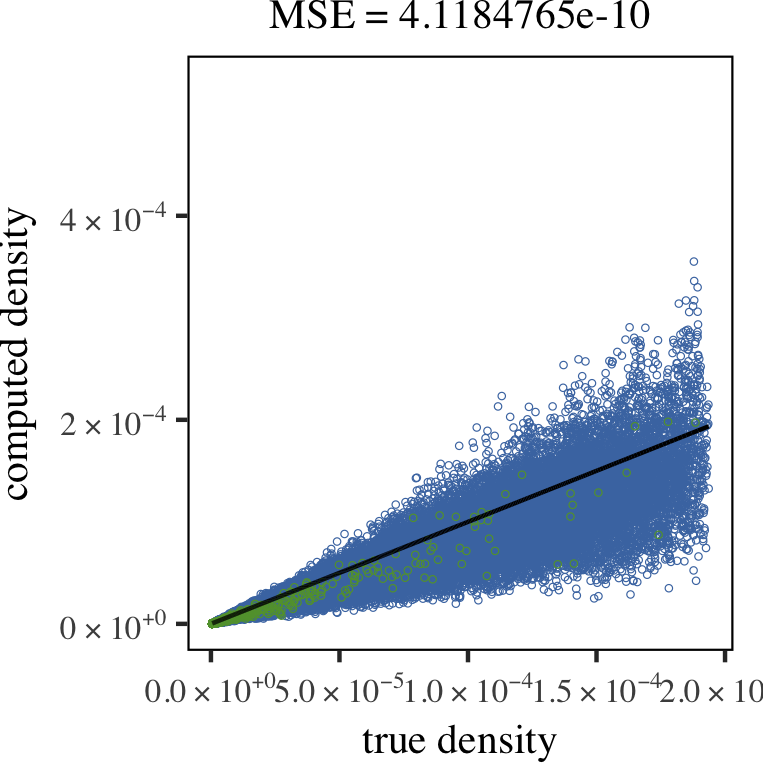
\includegraphics[keepaspectratio=true, width=\textwidth, height=0.23\textheight]{result/img/all/results_ferdosi_1_60000_mbe_silverman}
	\caption{Set \ferdosiOne, \mbe}
	\label{fig:results:singlesphere:mbe:ferdosi1}
\end{subfigure}
% Baakman 1	- MBE
\begin{subfigure}{0.23\textwidth}
	\centering
	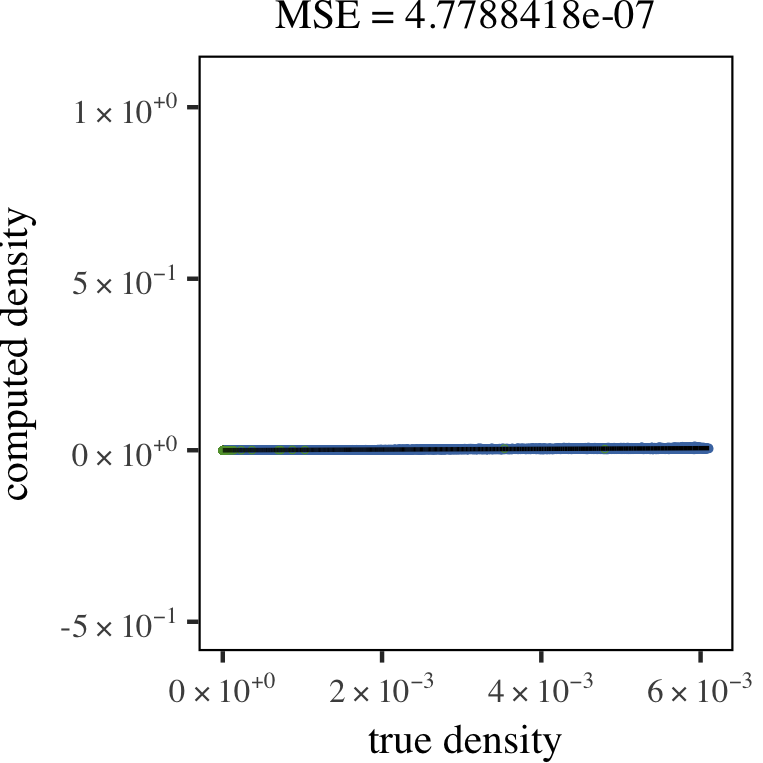
\includegraphics[keepaspectratio=true, width=\textwidth, height=0.23\textheight]{result/img/all/results_baakman_1_60000_mbe_silverman}
	\caption{Set \baakmanOne, \mbe}
	\label{fig:results:singlesphere:mbe:baakman1}
\end{subfigure}
% Baakman 4 - MBE
\begin{subfigure}{0.23\textwidth}
	\centering
	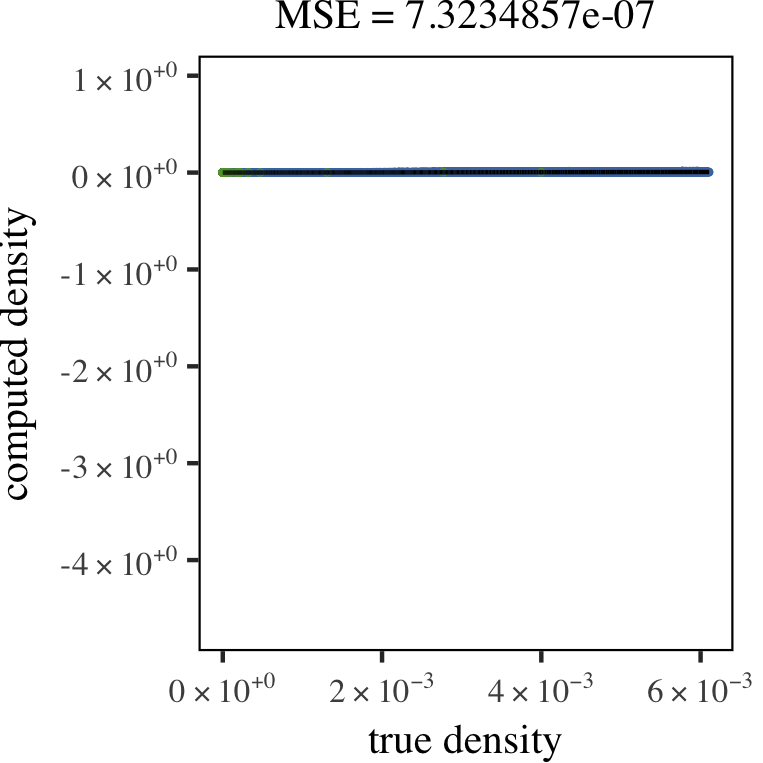
\includegraphics[keepaspectratio=true, width=\textwidth, height=0.23\textheight]{result/img/all/results_baakman_4_60000_mbe_silverman}
	\caption{Set \baakmanFour, \mbe}
	\label{fig:results:singlesphere:mbe:baakman4}
\end{subfigure}	
% Baakman 5 - MBE
\begin{subfigure}{0.23\textwidth}
	\centering
	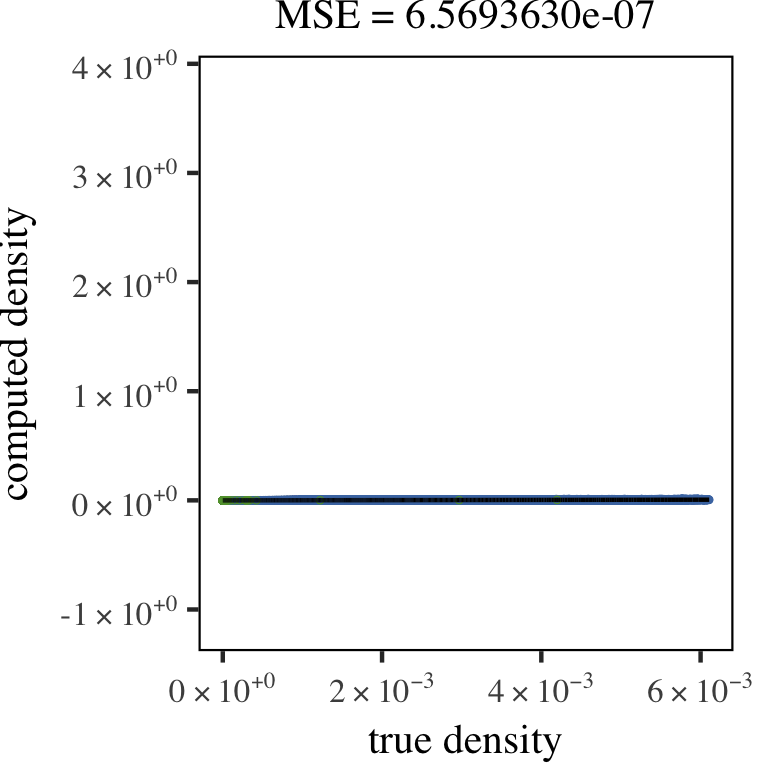
\includegraphics[keepaspectratio=true, width=\textwidth, height=0.23\textheight]{result/img/all/results_baakman_5_60000_mbe_silverman}
	\caption{Set \baakmanFive, \mbe}
	\label{fig:results:singlesphere:mbe:baakman5}
\end{subfigure}
% Ferdosi 1 - SAMBE
\begin{subfigure}{0.23\textwidth}
	\centering
	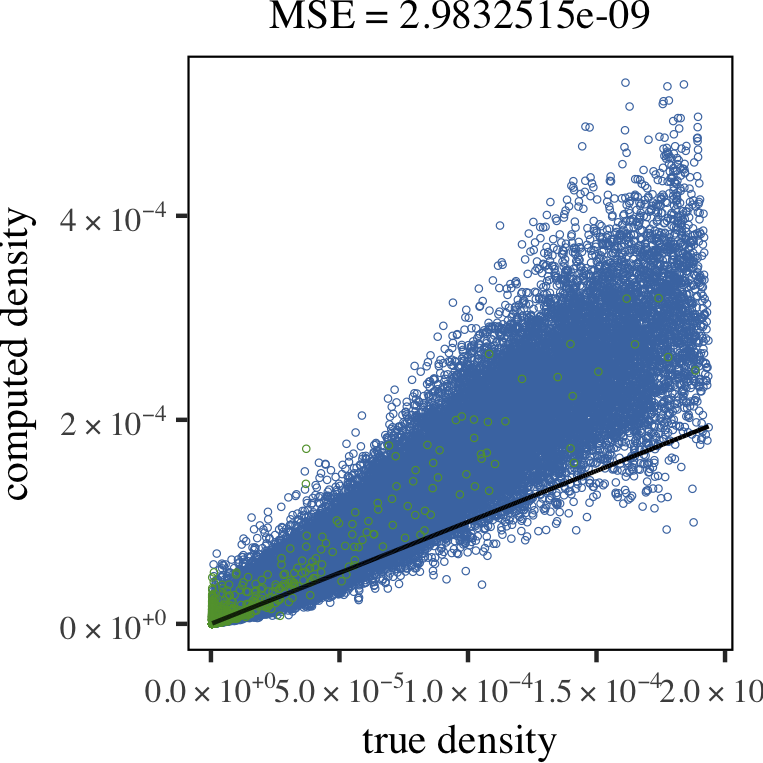
\includegraphics[keepaspectratio=true, width=\textwidth, height=0.23\textheight]{result/img/all/results_ferdosi_1_60000_sambe_silverman}
	\caption{Set \ferdosiOne, \sambe}
	\label{fig:results:singlesphere:sambe:ferdosi1}
\end{subfigure}
% Baakman 1	- SAMBE
\begin{subfigure}{0.23\textwidth}
	\centering
	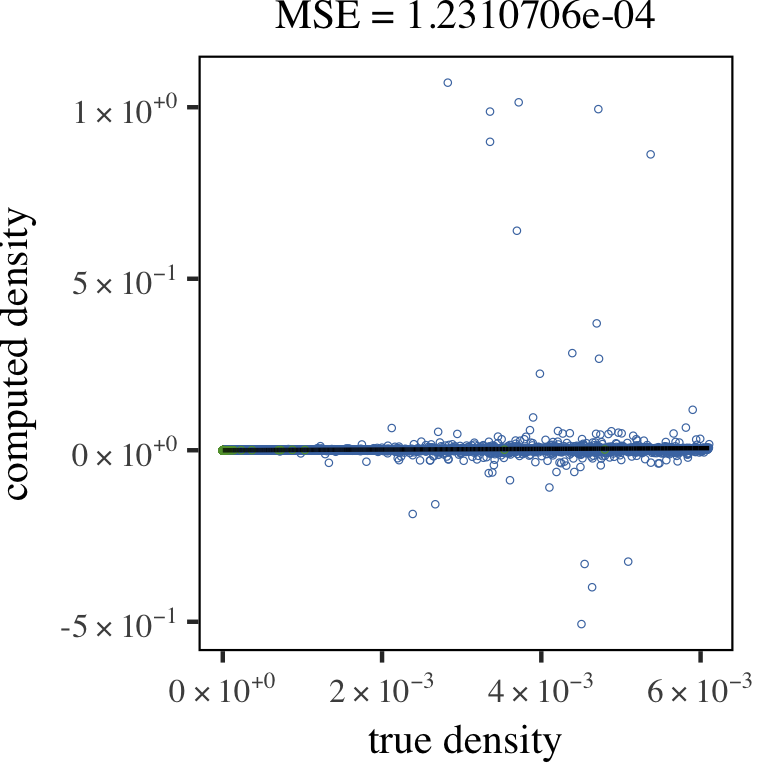
\includegraphics[keepaspectratio=true, width=\textwidth, height=0.23\textheight]{result/img/all/results_baakman_1_60000_sambe_silverman}
	\caption{Set \baakmanOne, \sambe}
	\label{fig:results:singlesphere:sambe:baakman1}
\end{subfigure}
% Baakman 4 - SAMBE
\begin{subfigure}{0.23\textwidth}
	\centering
	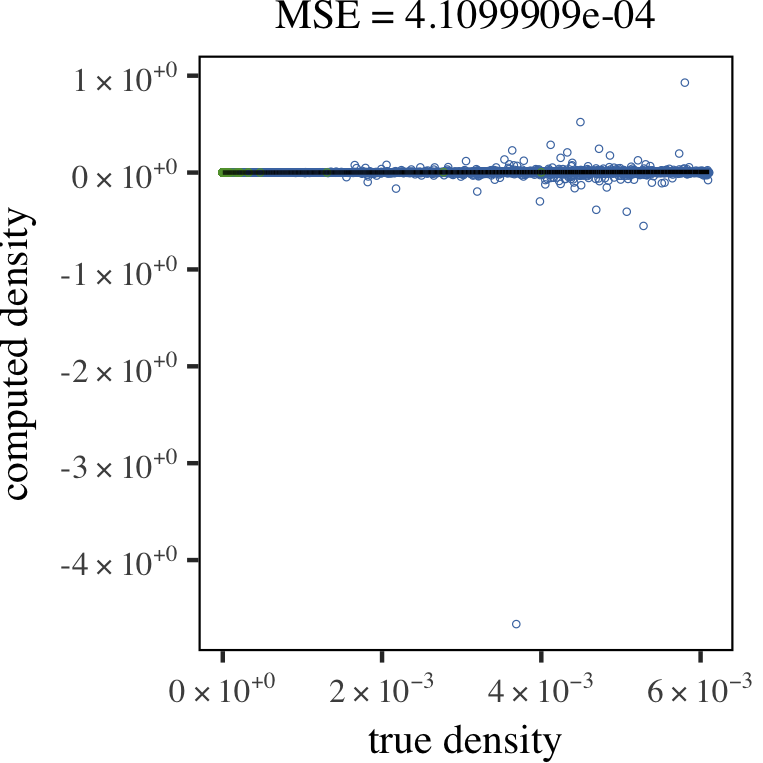
\includegraphics[keepaspectratio=true, width=\textwidth, height=0.23\textheight]{result/img/all/results_baakman_4_60000_sambe_silverman}
	\caption{Set \baakmanFour, \sambe}
	\label{fig:results:singlesphere:sambe:baakman4}
\end{subfigure}		
% Baakman 5 - SAMBE
\begin{subfigure}{0.23\textwidth}
	\centering
	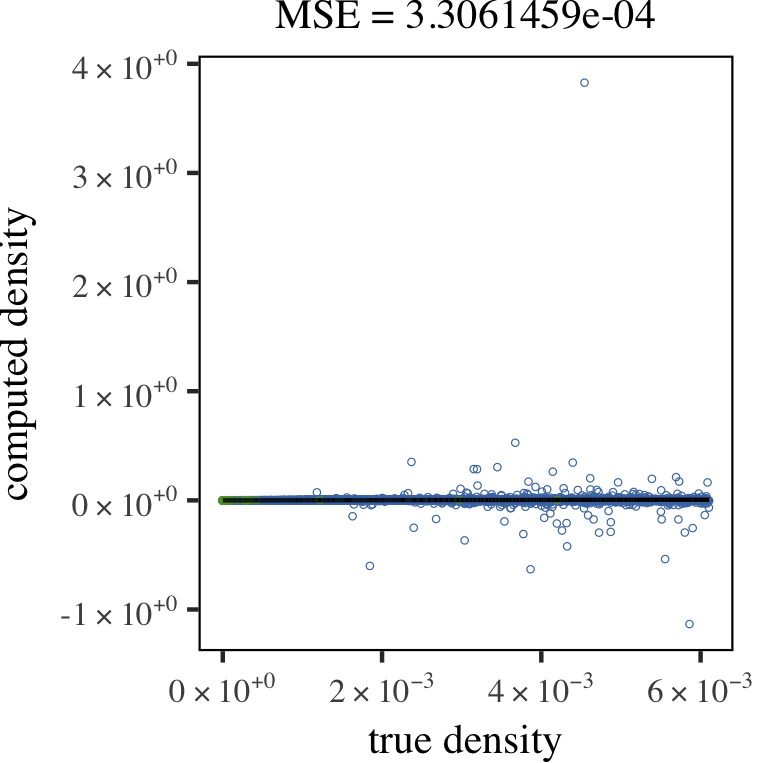
\includegraphics[keepaspectratio=true, width=\textwidth, height=0.23\textheight]{result/img/all/results_baakman_5_60000_sambe_silverman}
	\caption{Set \baakmanFive, \sambe}
	\label{fig:results:singlesphere:sambe:baakman5}
\end{subfigure}	
	\caption{Comparative plots for dataset \ferdosiOneNum, \baakmanOneNum, \baakmanFourNum, and \baakmanFiveNum.
	}
	\label{fig:results:singleSphere:comparativePlots}
\end{figure*}

\begin{table}
	\todo[inline]{Rewrite caption}
	\centering
	%!TEX root = ../paper.tex
\begin{tabular}{l*{2}{S[scientific-notation=true, round-mode=places,round-precision=3]}}
\toprule
~ 				& \multicolumn{2}{c}{Estimator}\\ \cmidrule{2-3}
Set				& {\mbe}					& {\sambe}	\\
\midrule
\ferdosiOne		& 0.0	&  0.0 \\
\baakmanOne		& 0.0	&  0.0 \\	
\baakmanFour	& 0.0	&  0.0 \\	
\baakmanFive	& 0.0	&  0.0 \\	
\bottomrule
\end{tabular}
	\caption{The mean squared error of the known densities and the densities as estimated by the Modified Breiman Estimator (\mbe) and the shape-adaptive MBE (\sambe), respectively, for the datasets containing a single Gaussian.} 	
	\label{tab:results:singleSphere:mse}
\end{table}

This section compares the performance of the Modified Breiman Estimator and a shape-adaptive variant on dataset that contain one Gaussian, \ie dataset \ferdosiOne, \baakmanOne, \baakmanFour, and \baakmanFive.

\todo[inline]{Where to find table and MSE?}

	% Ferdosi 1
		\todo[inline]{Discuss MSE and Plot}
		\todo[inline]{Difference between noise and gaussian?}

	% Baakman 1
		\todo[inline]{Discuss MSE and Plot}
		\todo[inline]{Difference between noise and gaussian?}

	% Baakman 4
		\todo[inline]{Discuss MSE and Plot}
		\todo[inline]{Difference between noise and gaussian?}

	% Baakman 5
		\todo[inline]{Discuss MSE and Plot}
		\todo[inline]{Difference between noise and gaussian?}

	% Algehele observatie voor single sphere datsets
		\todo[inline]{General observation}